\clearpage
\section{Reduced-form confounding-sensitivity extension}
\label{sec:confounding-supp}

\subsection{Identification and attribution}

This section develops the density-score estimation and covariance propagation for the fixed-error-correlation sensitivity identity of Imai, Keele and Yamamoto (2010), as cited in the main article. Let $m_t(\bX)=\alpha_2+\beta_2t+\bm\xi_2\trans\bX$ and $q_t(\bX)=a_t+\bm d_t\trans\bX$. A sufficient structural formulation is
\[
M(t)=m_t(\bX)+U_t,\qquad
Y(t,m)=q_t(\bX)+b_t\{m-m_t(\bX)\}+E_t.
\]
Assume treatment exchangeability conditional on baseline $\bX$, consistency and positivity; $U_t,E_t$ have conditional mean zero; and $E_t$ is invariant to the intervention value $m$. The sensitivity model allows mediator--outcome dependence through the joint law of $U_t$ and $E_t$. The observed reduced-form error is $W_t=b_tU_t+E_t$. Its conditional variance and covariance with $U_t$ obey
\[
\omega_t=b_tv_M+\rho_t\sqrt{v_M\Var(E_t)},\quad
v_t=b_t^2v_M+\Var(E_t)+2b_t\rho_t\sqrt{v_M\Var(E_t)}.
\]
Solving with positive $\Var(E_t)$ yields the main article's sensitivity slope. The natural indirect effect is $b_t\E\{M(1)-M(0)\}=b_t\beta_2$, since the additive $E_t$ cancels in the difference of nested potential outcomes. The total effect is $\E(q_1-q_0)$, giving the direct effects by the two decomposition identities. Thus the linear structural form supplies the causal interpretation and defines the sensitivity class: additive mediator--outcome confounding with an intervention-invariant structural error and a stratum-specific constant mediator slope.

For estimation, $U=M-m_T(\bX)$ has a common law independent of $(T,\bX)$, and the joint law of $(U,W_t)$ is stable across $\bX$ within each stratum. These assumptions support pooled-mediator and stratum-specific reduced-outcome fits with unspecified marginal densities. The figures follow the common-$\rho$ path through $(\rho_0,\rho_1)$.

\subsection{Estimating equations and covariance}

Let $S_M$ be the marginal regression score for $M$ on $(1,T,\bX\trans)$ and $S_{W_t}$ the score for $Y$ on $(1,\bX\trans)$ within $T=t$. The stacked population function is
\[
\Psi_i(\theta)=\begin{pmatrix}
S_{M,i}\\
1(T_i=0)S_{W_0,i}\\
1(T_i=1)S_{W_1,i}\\
1(T_i=0)(U_iW_{0i}-\omega_0)\\
1(T_i=1)(U_iW_{1i}-\omega_1)\\
\bX_i-\bmu_X
\end{pmatrix}.
\]
The first three blocks use the density-score equations and numerical settings in the main article. The OLS benchmark replaces each regression block by $(D e, e^2/v-1)$, with parameters $(\beta,\log v)$, so both methods estimate the same coefficient and variance nuisance parameters. Cross-covariances are the sample averages of fitted residual products within treatment groups. The parameter domain requires $v_Mv_t-\omega_t^2>0$; fitted values outside this domain are recorded transparently as numerical failures rather than altered by truncation.

Let $\widehat A=n^{-1}\sum_i\partial\widehat\Psi_i/\partial\theta\trans$ and $\widehat B=n^{-1}\sum_i\widehat\Psi_i\widehat\Psi_i\trans$. Within-stratum regression bread blocks are multiplied by $n_t/n$. The cross-product row for stratum $t$ has derivatives
\[
-n^{-1}\sum_{i:T_i=t}D_{Mi}\widehat W_{ti},\qquad
-n^{-1}\sum_{i:T_i=t}D_{Wi}\widehat U_i,
\]
with respect to the mediator and corresponding reduced-outcome coefficients, respectively, and derivative $-n_t/n$ with respect to $\omega_t$. It has zero direct derivative with respect to log variances. The baseline-mean block has bread $-I$. Empirical off-diagonal bread entries are retained even where their population expectations vanish. The full meat includes cross-covariance between the marginal regression scores and residual-product moments. The implemented covariance is $\widehat A^{-1}\widehat B\widehat A^{-\mathsf T}/n$.

\paragraph{Conditional asymptotic justification.}
Assume positive treatment probabilities and nonsingular bread. Also require finite score second moments and fourth error moments, and $v_Mv_t>\omega_t^2$. Each fitted marginal regression is assumed to satisfy the marginal analogues of Conditions~(\ref{cond:score-model})--(\ref{cond:score-derivative}) in Section~\ref{sec:regularity}. Require covariance consistency as in Condition~(\ref{cond:covariance}) for the full augmented stack, retaining its cross-block dependence rather than imposing the independent-error factorization used for the original mediation model. On any fixed finite collection of sensitivity values strictly inside $(-1,1)$, the marginal expansions hold jointly. Taylor expansion of the appended residual-product equations and empirical baseline mean then gives the stacked expansion $\varphi_\theta=-A^{-1}\Psi$. Applying the chain rule gives $\varphi_{g,\rho}=G_\rho\varphi_\theta$ and the displayed sandwich covariance. Positive effect variance is required for a scalar Wald interval. Thus standard estimating-equation and delta-method theory supplies pointwise asymptotic inference under the stated marginal-estimator regularity. The efficiency interpretation is attached to the marginal score blocks; the displayed joint representation characterizes the assembled estimator in the reduced-form working model.

\subsection{Analytic gradients and zero boundaries}

Put $\ell_t=\omega_t/v_M$, $A_t=v_t/v_M$, $d_t=\sqrt{A_t-\ell_t^2}$ and $h_t=\rho_t/\sqrt{1-\rho_t^2}$. Then $b_t=\ell_t-h_td_t$ and
\begin{align*}
\frac{\partial b_t}{\partial\omega_t}&=\frac{1+h_t\ell_t/d_t}{v_M},\\
\frac{\partial b_t}{\partial\log v_M}&=-\ell_t+\frac{h_t(A_t-2\ell_t^2)}{2d_t},\\
\frac{\partial b_t}{\partial\log v_t}&=-\frac{h_tA_t}{2d_t}.
\end{align*}
Thus $d\delta_t=b_t\,d\beta_2+\beta_2\,db_t$. For the total effect,
\[
d\tau=d(a_1-a_0)+\bmu_X\trans d(\bm d_1-\bm d_0)
+(\bm d_1-\bm d_0)\trans d\bmu_X.
\]
Direct-effect gradients are obtained by subtraction. The code supports separate $(\rho_0,\rho_1)$ even though the figures use their common-value path.

For $\beta_2\ne0$, $\delta_t(\rho_t)=0$ exactly at $r_t=\omega_t/\sqrt{v_Mv_t}$. Its derivatives are $\partial r_t/\partial\omega_t=1/\sqrt{v_Mv_t}$ and $\partial r_t/\partial\log v_M=\partial r_t/\partial\log v_t=-r_t/2$. We form a delta interval for $\operatorname{atanh}(r_t)$ and transform its endpoints back with $\tanh$. At $\beta_2=0$, the complete indirect-effect curve equals zero, producing a set-valued rather than unique effect-zero threshold. The confidence interval for a unique zero boundary addresses uncertainty in the point-estimate threshold, while the statistical-significance boundary along the curve addresses pointwise interval exclusion of zero.

Under the working error independence from regressors, the first-order derivatives of residual second moments with respect to the mean coefficients vanish. Their influence terms reduce to $U^2-v_M$, $1(T=t)(W_t^2-v_t)/p_t$ and $1(T=t)(UW_t-\omega_t)/p_t$. Consequently the OLS-RF and DS-RF zero-boundary estimators share the same first-order residual-moment representation under this model, explaining their close finite-sample boundaries. Density-score gains for the indirect-effect curve arise instead through the pooled mediator treatment coefficient and its joint covariance with the remaining nuisance estimates.

For the contour calibration, Imai's additional shared-confounder variance decomposition expresses $U$ and $E_t$ as linear contributions of a hypothetical pretreatment confounder plus uncorrelated remainder errors, with the corresponding orthogonality to the confounder. It gives $\rho_t^2=R_M^{2*}R_{Y,t}^{2*}$, with the sign specified separately. The outcome fraction refers to the \emph{structural outcome error}, which is distinct from the observed reduced-form outcome residual. The figure uses this moment calibration to map hypothetical latent variance fractions into sensitivity values without requiring a complete latent distribution. Accordingly, its axes are labeled as residual-variance fractions rather than total-variance tilde quantities.

\subsection{Simulation design and verification}

The main article's confounding experiment uses seed 20260918, $n=300$ and 500 replications per innovation-by-correlation cell. For independent verification, the stratum-$t$ covariance is $-0.8+t+\rho_{\rm true}$ and the reduced-outcome variance is $(-0.8+t+\rho_{\rm true})^2+1-\rho_{\rm true}^2$; these determine the population zero boundaries. The original natural effects are retained. Evaluation at the generating correlation and at zero includes valid-fit, paired-fit and all-attempted summaries, with every fit status recorded.

Table~\ref{tab:confounding-simulation} gives performance at the generating correlation; the full-curve and zero-boundary assessments follow below. JOBS II curves are grouped with the application in Section~\ref{sec:jobs}.

\begin{table}[htbp]\centering\small\setlength{\tabcolsep}{3pt}
\caption{Reduced-form sensitivity estimation at the true structural correlation: $n=300$, 500 attempts per cell. Coverage and precision use valid fits; Success uses all attempts.}
\label{tab:confounding-simulation}
\begin{tabular}{lrllrrrrr}\toprule
Error & $\rho$ & Effect & Method & Bias & RMSE & Coverage (MCSE) & Length & Success\\\midrule
AM & -0.3 & PNIE & OLS-RF & 0.017 & 0.067 & 0.966 (0.008) & 0.257 & 1.000\\
AM & -0.3 & PNIE & DS-RF & 0.000 & 0.066 & 0.958 (0.009) & 0.260 & 0.996\\
AM & -0.3 & TE & OLS-RF & -0.011 & 0.145 & 0.950 (0.010) & 0.560 & 1.000\\
AM & -0.3 & TE & DS-RF & -0.011 & 0.145 & 0.946 (0.010) & 0.560 & 0.996\\
AM & 0.0 & PNIE & OLS-RF & 0.003 & 0.070 & 0.946 (0.010) & 0.283 & 1.000\\
AM & 0.0 & PNIE & DS-RF & 0.002 & 0.049 & 0.952 (0.010) & 0.198 & 1.000\\
AM & 0.0 & TE & OLS-RF & -0.004 & 0.128 & 0.964 (0.008) & 0.527 & 1.000\\
AM & 0.0 & TE & DS-RF & -0.004 & 0.127 & 0.968 (0.008) & 0.527 & 1.000\\
AM & 0.3 & PNIE & OLS-RF & 0.011 & 0.079 & 0.974 (0.007) & 0.324 & 1.000\\
AM & 0.3 & PNIE & DS-RF & 0.001 & 0.044 & 0.946 (0.010) & 0.170 & 0.998\\
AM & 0.3 & TE & OLS-RF & -0.002 & 0.124 & 0.960 (0.009) & 0.490 & 1.000\\
AM & 0.3 & TE & DS-RF & -0.002 & 0.124 & 0.958 (0.009) & 0.490 & 0.998\\
\midrule
G & -0.3 & PNIE & OLS-RF & 0.004 & 0.108 & 0.926 (0.012) & 0.418 & 1.000\\
G & -0.3 & PNIE & DS-RF & 0.005 & 0.110 & 0.924 (0.012) & 0.434 & 1.000\\
G & -0.3 & TE & OLS-RF & 0.000 & 0.146 & 0.932 (0.011) & 0.558 & 1.000\\
G & -0.3 & TE & DS-RF & 0.000 & 0.146 & 0.934 (0.011) & 0.558 & 1.000\\
G & 0.0 & PNIE & OLS-RF & 0.004 & 0.102 & 0.946 (0.010) & 0.397 & 1.000\\
G & 0.0 & PNIE & DS-RF & 0.003 & 0.105 & 0.946 (0.010) & 0.413 & 1.000\\
G & 0.0 & TE & OLS-RF & 0.001 & 0.140 & 0.940 (0.011) & 0.529 & 1.000\\
G & 0.0 & TE & DS-RF & 0.001 & 0.140 & 0.942 (0.010) & 0.529 & 1.000\\
G & 0.3 & PNIE & OLS-RF & 0.005 & 0.098 & 0.940 (0.011) & 0.385 & 1.000\\
G & 0.3 & PNIE & DS-RF & 0.005 & 0.102 & 0.938 (0.011) & 0.402 & 1.000\\
G & 0.3 & TE & OLS-RF & -0.000 & 0.119 & 0.962 (0.009) & 0.490 & 1.000\\
G & 0.3 & TE & DS-RF & -0.000 & 0.119 & 0.962 (0.009) & 0.491 & 1.000\\
\bottomrule\end{tabular}
\par\smallskip\begin{minipage}{0.98\textwidth}\footnotesize G: Gaussian; AM: asymmetric mixture. OLS-RF and DS-RF use the same reduced-form models with OLS and marginal density-score regression, respectively. They are not the conditional-outcome estimators in the original simulation. All five effects, zero-rho analyses, threshold inference and paired comparisons are retained in the project repository.\end{minipage}
\end{table}


The independent tests compare analytic and numerical gradients for all five effects, verify both exact decompositions and covariance symmetry, reconstruct the Imai covariance identity at known population parameters, and check zero-boundary derivatives and separate-correlation inputs. Output checks independently recompute performance summaries, compare paired replication identifiers, check all attempted/valid denominators, and reconstruct retained OLS fits from the recorded seeds. The existing core estimator is unchanged.

\clearpage
\subsection{Full-curve Monte Carlo assessment}

The full-curve evaluation reconstructs the same 3,000 data sets and estimator settings from the stored seeds, as recorded in \path{CURVE_SIMULATION_PLAN_20260916.md}. Each fit supplies five effects on $\{-0.8,-0.75,\ldots,0.8\}$. With generating correlation $r$, the moments $v_M=1$, $\omega_t=-0.8+t+r$ and $v_t=\omega_t^2+1-r^2$ give the main article's population curve. The total effect is 0.78 throughout; direct effects follow by subtraction.

For assumed $\rho$, bias, RMSE and coverage target the population sensitivity functional; \texttt{CausalBias} and \texttt{CausalInclusion} target the generating causal effect. Paired ratios use common valid replication identifiers. Monte Carlo calculations preserve within-curve dependence and use the valid-fit or all-attempt denominators defined in Section~\ref{sec:paired-audit}.

For a common assumed correlation, write $h=\rho/\sqrt{1-\rho^2}$. Each fitted effect has the exact form
\[
\widehat g(\rho)=\widehat A+h\widehat B,\qquad
\widehat\Var\{\widehat g(\rho)\}
=\widehat V_A+2h\widehat C_{AB}+h^2\widehat V_B.
\]
Here $A=g(\theta;0)$ and $B=g(\theta;1/\sqrt2)-g(\theta;0)$, with gradients obtained from the previously displayed effect map. The covariance terms follow jointly from the complete nuisance sandwich. The project repository stores these five coefficients for every effect and attempted fit, allowing all grid values and intervals to be reconstructed exactly for any plotting grid without refitting, smoothing or interpolating confidence limits. Unsuccessful fits retain missing coefficients and a diagnostic message.

The main figure's central 90\% empirical ranges describe the sampling distribution of the effect estimates across valid fits. Figure~\ref{fig:curve-coverage} separately evaluates each fit's nominal 95\% pointwise interval, and Figure~\ref{fig:curve-ratios} compares RMSE on paired valid data sets. Reading the RMSE ratios together with pointwise coverage is particularly informative where the estimated curve is near zero. Table~\ref{tab:curve-thresholds} adds a distinct evaluation of the estimated point-effect zero boundary.

\begin{figure}[p]
\centering
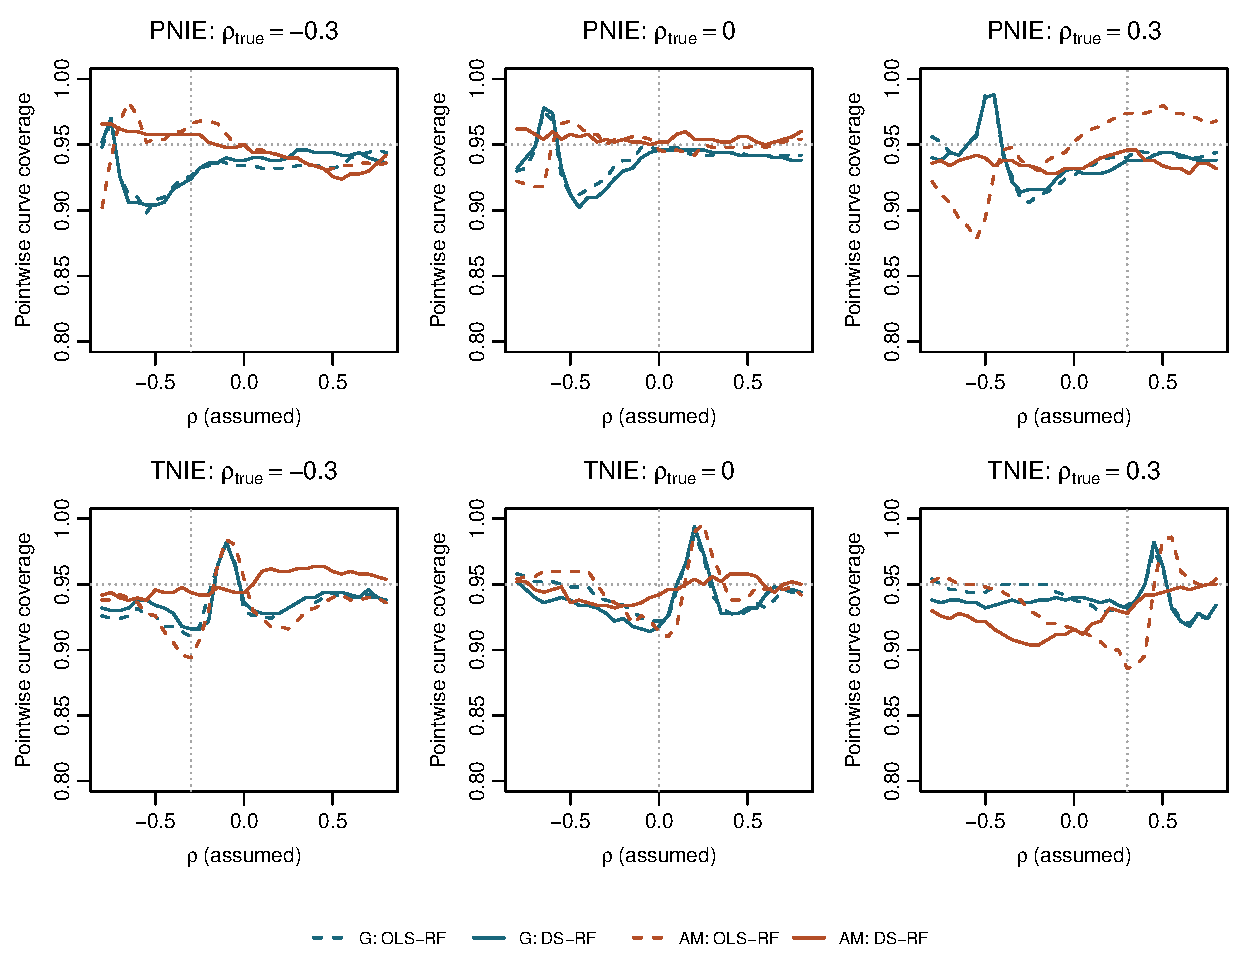
\includegraphics[width=0.98\textwidth]{figures/confounding_simulation_curve_coverage.pdf}
\caption{Pointwise coverage of the population sensitivity functional across the full assumed-correlation grid, conditional on numerical success. Each configuration starts with 500 attempts. G denotes Gaussian innovations and AM asymmetric-mixture innovations. The horizontal line is 0.95 and the vertical line is the generating correlation. At other correlations, coverage targets the corresponding sensitivity functional; at the generating correlation, that functional equals the generating causal effect. Complete Monte Carlo standard errors and report-and-cover fractions are retained in the project repository.}
\label{fig:curve-coverage}
\end{figure}

\begin{figure}[p]
\centering
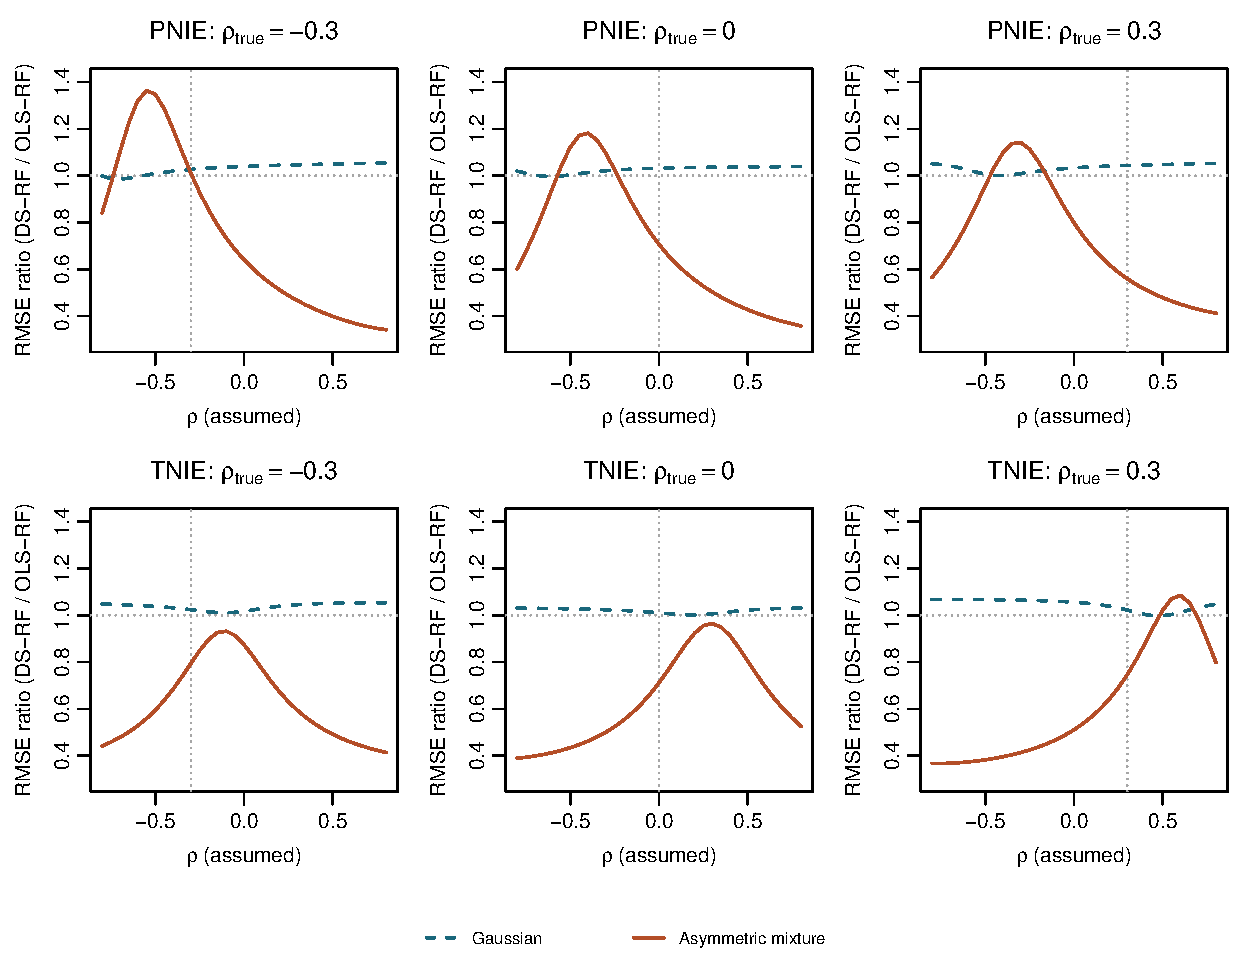
\includegraphics[width=0.98\textwidth]{figures/confounding_simulation_curve_ratios.pdf}
\caption{Paired DS-RF/OLS-RF RMSE ratios for the population PNIE/TNIE sensitivity curves. Ratios below one favor DS-RF in RMSE. The same successful data sets are used in the numerator and denominator, and all assumed correlations and generating configurations are retained. Pointwise coverage and numerical success provide the complementary calibration and reliability measures.}
\label{fig:curve-ratios}
\end{figure}

\begin{table}[htbp]\centering\small\setlength{\tabcolsep}{4pt}
\caption{Zero-boundary inference in the confounding simulation. The same retained data sets are used; these are not additional independent replications. Coverage and length refer to the Fisher-transform interval for $\rho_t^\dagger$.}
\label{tab:curve-thresholds}
\begin{tabular}{lrllrrrr}\toprule
Error & $\rho_{\rm true}$ & Effect & Method & Bias & RMSE & Coverage (MCSE) & Length\\\midrule
AM & -0.3 & PNIE & OLS-RF & 0.003 & 0.068 & 0.958 (0.009) & 0.276\\
AM & -0.3 & PNIE & DS-RF & 0.004 & 0.068 & 0.960 (0.009) & 0.275\\
AM & -0.3 & TNIE & OLS-RF & 0.001 & 0.078 & 0.940 (0.011) & 0.311\\
AM & -0.3 & TNIE & DS-RF & 0.002 & 0.077 & 0.944 (0.010) & 0.311\\
AM & 0.0 & PNIE & OLS-RF & 0.006 & 0.072 & 0.958 (0.009) & 0.290\\
AM & 0.0 & PNIE & DS-RF & 0.006 & 0.072 & 0.960 (0.009) & 0.290\\
AM & 0.0 & TNIE & OLS-RF & 0.008 & 0.081 & 0.946 (0.010) & 0.311\\
AM & 0.0 & TNIE & DS-RF & 0.007 & 0.081 & 0.944 (0.010) & 0.312\\
AM & 0.3 & PNIE & OLS-RF & -0.002 & 0.079 & 0.950 (0.010) & 0.306\\
AM & 0.3 & PNIE & DS-RF & -0.002 & 0.079 & 0.950 (0.010) & 0.305\\
AM & 0.3 & TNIE & OLS-RF & -0.003 & 0.080 & 0.936 (0.011) & 0.301\\
AM & 0.3 & TNIE & DS-RF & -0.004 & 0.079 & 0.936 (0.011) & 0.301\\
\midrule
G & -0.3 & PNIE & OLS-RF & 0.002 & 0.058 & 0.950 (0.010) & 0.215\\
G & -0.3 & PNIE & DS-RF & 0.002 & 0.058 & 0.948 (0.010) & 0.215\\
G & -0.3 & TNIE & OLS-RF & 0.002 & 0.080 & 0.954 (0.009) & 0.311\\
G & -0.3 & TNIE & DS-RF & 0.002 & 0.080 & 0.952 (0.010) & 0.311\\
G & 0.0 & PNIE & OLS-RF & 0.006 & 0.063 & 0.946 (0.010) & 0.243\\
G & 0.0 & PNIE & DS-RF & 0.006 & 0.063 & 0.946 (0.010) & 0.243\\
G & 0.0 & TNIE & OLS-RF & 0.005 & 0.081 & 0.944 (0.010) & 0.307\\
G & 0.0 & TNIE & DS-RF & 0.005 & 0.081 & 0.948 (0.010) & 0.307\\
G & 0.3 & PNIE & OLS-RF & 0.008 & 0.069 & 0.954 (0.009) & 0.274\\
G & 0.3 & PNIE & DS-RF & 0.008 & 0.069 & 0.954 (0.009) & 0.274\\
G & 0.3 & TNIE & OLS-RF & -0.000 & 0.069 & 0.946 (0.010) & 0.274\\
G & 0.3 & TNIE & DS-RF & -0.000 & 0.069 & 0.944 (0.010) & 0.274\\
\bottomrule\end{tabular}
\par\smallskip\begin{minipage}{0.98\textwidth}\footnotesize G: Gaussian; AM: asymmetric mixture. Each cell starts with 500 attempts. Success denominators and failure records are the same as for Table~\ref{tab:confounding-simulation}. A zero boundary of the point-estimate curve is not an interval-zero boundary.\end{minipage}
\end{table}


\clearpage

